%----------------------------------------------------------------------------
\chapter{次世代ピクセル検出器の量産}
\label{sec:singatapixel-devel}
%----------------------------------------------------------------------------
〜と同時に、HL-LHCアップグレードに向けた内部飛跡検出器の総入れ替えのため、次世代ピクセル検出器の開発が進められている。現在、ITkに搭載するピクセル検出器量産の各組み立て工程における試験やそのシステムの確立のため、試作器を用いたデモンストレーションが行われている。

日本では新型器量産の際に約$2000$個のモジュールを生産する予定である。新型器の量産の際に、効率の良い量産と統合されたモジュール選定を行うため、品質試験結果を統合管理するシステムの開発が必要となる。


%----------------------------------------------------------------------------
\section{次世代ピクセル検出器の組み立て部品}
\label{sec:component}
%----------------------------------------------------------------------------
量産工程は、各組み立て機関に届いたセンサーとASICから作られるベアモジュールとフレキシブル基板の接着から始まる。本節では各部品の詳細について説明する。


%----------------------------------------------------------------------------
\subsection{ベアモジュール}
\label{sec:bare}
%----------------------------------------------------------------------------

ベアモジュールはセンサーとASICをバンプ接合することにより作られる。クアッドモジュールではセンサー1枚に対してASIC4枚、トリプレットモジュールではセンサー1枚に対してASIC1枚から構成される。ベアモジュールは通過する粒子を検出する、モジュールの中でも重要な部品である。センサーを通過した荷電粒子は電子・ホール対を生成し、それにより得られる信号をASICを用いて増幅・整形を行う。\fref{fig:bare}にベアモジュールの全体図を示す。
\begin{figure}[tbp]
  \centering
  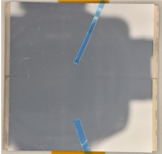
\includegraphics[height=5cm,keepaspectratio]{bare.png}
  \caption[ベアモジュール]{ベアモジュールの全体図。センサー側から見たものであり、左右にASICがはみ出している。これはフレキシブル基板につながるワイヤーのためのパッドが存在する部分である。}
  \label{fig:bare}
\end{figure}

%現在行われている試作器の組み立てではRD53AというASICを用いている。


%----------------------------------------------------------------------------
\subsection{フレキシブル基板}
\label{sec:flex}
%----------------------------------------------------------------------------

フレキシブル基板はセンサーの裏側(\fref{fig:bare}ので見えている面)に接着され、

\begin{figure}[tbp]
  \centering
  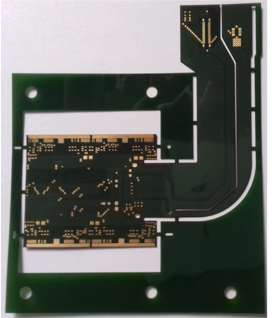
\includegraphics[height=6cm,keepaspectratio]{flex.png}
  \caption[フレックス基板]{フレックス基板の全体図。}
  \label{fig:flex}
\end{figure}

フレキシブル基板は、以下の3つの役割を持つ。
\begin{itemize}
  \item ASICからの信号輸送  \\
  センサーから得られた信号はASICで増幅・整形され、フレキシブル基板に送られてくる。フレキシブル基板は送られてきた信号を後段のPCへ送る。
  \item 電源の供給 \\
  外部からの電源を、センサーとASICに供給する。センサーには、空乏領域を増加させるために$100\ \si{V}$程度のHV(\textbf{H}igh \textbf{V}oltage)をかける。ASICには、電源供給のために$5.6\ \si{V}$程度のLV(\textbf{L}ow \textbf{V}oltage)
  \item モジュールの制御システム(DCS: \textbf{D}etector \textbf{C}ontrol \textbf{S}ystem) \\
  モジュールの温度測定のために2つのNTC(\textbf{N}egative \textbf{T}emperature \textbf{C}oefficient)が配置されている。
\end{itemize}

%----------------------------------------------------------------------------
\subsection{モジュールキャリア}
\label{sec:carrier}
%----------------------------------------------------------------------------

モジュールキャリアはモジュールの運搬の際や品質試験を行う際に、モジュールを保護用の容器である。組み立てられたモジュールはASICとフレックス基板を繋ぐワイヤー部やセンサーの部分等が剥き出しになっているため、そのままの状態で品質試験を行うのはモジュール破損のリスクを伴う。モジュールキャリアでモジュールを保護することにより、安全に品質試験を行うことができる。

また、モジュールキャリアの別の役割として、モジュール周囲の湿度環境を一定に保つことが挙げられる。運転時に想定される最低温度は$-45\ \si{\degreeCelsius}$のため、品質管理試験ではペルチェ素子を用いた温度制御装置\footnote{KEKにおける次世代ピクセル検出器の量産では、東工大を中心に開発している温度制御システムを用いる。}を用いて$-45\ \si{\degreeCelsius}$までモジュールの周囲温度を下げる。その際、モジュールへの結露を防ぐための結露を防ぐためキャリア内に乾燥窒素ガスを流し込むことで氷点下においてもモジュールへの結露を防いでいる。

%----------------------------------------------------------------------------
\section{次世代ピクセル検出器の組み立て工程}
\label{sec:assemble}
%----------------------------------------------------------------------------
\begin{figure}[tbp]
  \centering
  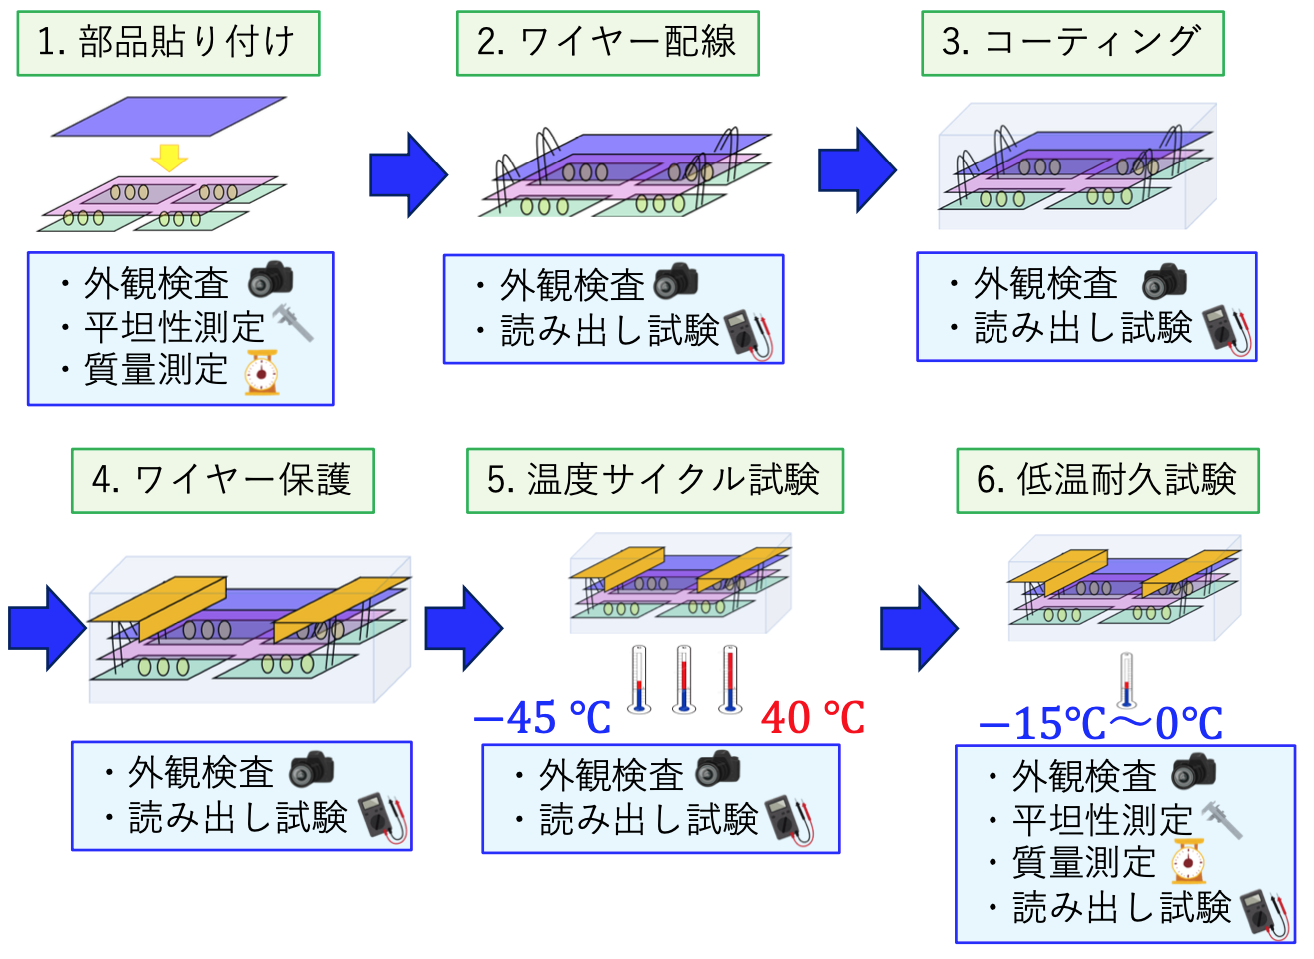
\includegraphics[height=7cm,keepaspectratio]{module_flow.png}
  \caption[ATLAS検出器]{ATLAS検出器の全体図 \cite{studyofID} }
  \label{fig:assemble}
\end{figure}


次世代ピクセル検出器の組み立て工程を\fref{fig:assemble}に示す。組み立て工程ではフレキシブル基板とベアモジュールの接着から始まり、ワイヤー配線、パリレン高分子によるコーティング、ワイヤー保護を行いピクセルモジュールが完成する。その後、温度サイクル試験および低温耐久試験において、運転時に想定される温度環境において組み立てたモジュールが運用できるかの試験を行う。本節では、組み立て工程、およびモジュールの温度耐久についての試験についての説明を示す。

\subsubsection*{ベアモジュール・フレキシブル基板の接合}

モジュールの組み立て工程は、組み立て機関に輸送されたベアモジュールとフレキシブル基板の接合から始まる。輸送された各部品の外観検査等の受け取り時の試験を行った後、ベアモジュールとフレキシブル基板の接合を行う。接合の後、モジュールの外観検査・平坦性測定・質量測定を行う。

\subsubsection*{ワイヤー配線}

フレキシブル基板からセンサーおよびASICへの電圧の供給や、ASICからの信号を読み出すため、フレキシブル基板とセンサーおよびASIC間をワイヤーで接続する。

\subsubsection*{パリレンコーティング}

モジュールのセンサーとASICの端の部分での放電を防ぐこと、湿気や化学物質からの保護を目的としてパリレンコーティングを行う。パリレンはパラキシリレン系ポリマーの略である。パリレンは結晶性が高く絶縁耐力に優れ、周波数に依存せず低い誘電率・誘電正接特性を持っており、湿気や腐食性ガスへの耐性も併せ持つ。


\subsubsection*{ワイヤー保護}

ワイヤーは直径$25\ \si{\micro m}$のため、非常に細い。

\subsubsection*{温度サイクル}

組み立てたモジュールに対して、ITk実装後にされる特異的な温度変化のサイクルを行い、その後もモジュールが正常な応答をするか試験をする。温度変化の際、フレキシブル基板にたわみが生じ、それが原因でバンプ接合部に剥がれが生じてしまうことがある。このようの温度サイクルによるモジュールの損傷がないことを確認する必要がある。

温度サイクルは、動作温度範囲$-45\ \si{\degreeCelsius}<T<40\ \si{\degreeCelsius}$で$100$サイクル以上、$-55\ \si{\degreeCelsius}<T<60\ \si{\degreeCelsius}$を$1$サイクルである。

\subsubsection*{低温耐久試験}

ITk運転におけるピクセル検出器の周囲温度は$-15\ \si{\degreeCelsius}<T<0\ \si{\degreeCelsius}$である。組み立てたモジュールが低温環境下において長時間正常に動作することを確認する試験が低温耐久試験である。
低温耐久試験では、温度制御筐体を用いてモジュールの周囲温度を$-15\ \si{\degreeCelsius}$に保ちつつASICの回路読み出し試験を行う。読み出し試験は1時間に1度行われる。

長時間放置しつつ読み出し試験を行うため、インターロックシステム、機器の遠隔制御、温度制御筐体の遠隔監視等の技術が必要となる。


%----------------------------------------------------------------------------
\section{品質試験}
\label{sec:QCtest}
%----------------------------------------------------------------------------




\subsection{}

%----------------------------------------------------------------------------
\section{量産における試験結果管理}
\label{sec:}
%----------------------------------------------------------------------------



\newpage
